% Emacs, this is -*-latex-*-

\ex{Importance sampling to estimate tail probabilities {\small \citep[based on][Exercise 3.5]{Robert2010}}}
\label{ex:importance-sampling-to-estimate-tail-probabilities}
We would like to use importance sampling to compute the probability
that a standard Gaussian random variable $x$ takes on a value larger
than $5$, i.e
\begin{equation}
  \Pr(x>5) = \int_{5}^\infty \frac{1}{\sqrt{2\pi}} \exp\left(-\frac{x^2}{2}\right) dx
\end{equation}
We know that the probability equals
\begin{align}
  \Pr(x>5) & = 1-\int_{-\infty}^5 \frac{1}{\sqrt{2\pi}} \exp\left(-\frac{x^2}{2}\right) dx\\
  & = 1-\Phi(5)\\
  & \approx 2.87 \cdot 10^{-7}
\end{align}
where $\Phi(.)$ is the cumulative distribution function of a standard
normal random variable.

\begin{exenumerate}
\item With the indicator function $\mathbbm{1}_{x>5}(x)$, which
  equals one if $x$ is larger than $5$ and zero otherwise, we can
  write $\Pr(x>5)$ in form of the expectation
  \begin{align}
    \Pr(x>5) &= \E[ \mathbbm{1}_{x>5}(x) ],
  \end{align}
  where the expectation is taken with respect to the density
  $\mathcal{N}(x; 0, 1)$ of a standard normal random variable,
  \begin{equation}
    \mathcal{N}(x; 0, 1) = \frac{1}{\sqrt{2\pi}} \exp\left(-\frac{x^2}{2}\right).
  \end{equation}
  This suggests that we can approximate $\Pr(x>5)$ by a Monte Carlo average
  \begin{equation}
    \Pr(x>5) \approx \frac{1}{n} \sum_{i=1}^n \mathbbm{1}_{x>5}(x_i), \quad \quad \quad x_i \sim  \mathcal{N}(x; 0, 1).
  \end{equation}
  Explain why this approach does not work well.

  \begin{solution}
    In this  approach, we essentially  count how many times  the $x_i$
    are larger than  5. However, we know that the  chance that $x_i>5$
    is only  $2.87 \cdot 10^{-7}$. That  is, we only  get about one value above 5
    every 20 million simulations! The approach is thus very sample inefficient.

    \if0
    More formally, we can assess the variability of the estimate $\hat{I}_n$,
    \begin{equation}
      \hat{I}_n = \frac{1}{n} \sum_{i=1}^n \mathbbm{1}_{x>5}(x_i) \quad \quad x_i \sim  \mathcal{N}(x; 0, 1)
    \end{equation}
    One possibility is to compute the variance of $\hat{I}_n$. It equals
    \begin{align}
      \Var[ \hat{I}_n] = \frac{1}{n} \Var[\mathbbm{1}_{x>5}(x)]
    \end{align}
    The quantity $y = \mathbbm{1}_{x>5}(x)$ is a binary random
    variable taking on the value 0 (if $x\le 5$) or 1 (if $x >5$). It
    thus is a Bernoulli random variable with success probability $p$,
    i.e. the probability for $y=1$, being equal to the probability
    $\Pr(x>5)$. Hence, we can use the formula for the variance of a Bernoulli random variable which is
    \begin{align}
      \Var(y) &= p(1-p)\\
      & = \Pr(x>5)(1-\Pr(x>5))
    \end{align}
    Hence the variance $\Var[ \hat{I}_n]$ equals
    \begin{equation}
      \Var[ \hat{I}_n] = \frac{1}{n} \Pr(x>5)(1-\Pr(x>5))
    \end{equation}
    Since $\Pr(x>5)$ is very small, the variance is also very
    small. Hence, very often may want to assess the variability
    relative to the mean of the random variable. This is what the
    coefficient of variability is doing: it equals the standard
    deviation divided by the mean.  ...  (normalisation by n is also
    needed to assess the rate of convergence but this seems like too
    much of a digression. omit.
    \fi
  \end{solution}

\item Another approach is to use importance sampling with an importance distribution $q(x)$ that is zero for $x<5$. We can then write $\Pr(x>5)$ as
  \begin{align}
    \Pr(x>5) & = \int_{5}^\infty \frac{1}{\sqrt{2\pi}} \exp\left(-\frac{x^2}{2}\right) dx\\
    & = \int_{5}^\infty \frac{1}{\sqrt{2\pi}} \exp\left(-\frac{x^2}{2}\right) \frac{q(x)}{q(x)} dx \\
    & = \E_{q(x)} \left[\frac{1}{\sqrt{2\pi}} \exp\left(-\frac{x^2}{2}\right) \frac{1}{q(x)}\right]
  \end{align}
  and estimate $\Pr(x>5)$ as a sample average.
  
  We here use an exponential distribution shifted by $5$ to the right. It has pdf
  \begin{equation}
    q(x) = \begin{cases}
      \exp(- (x-5)) & \text{if } x\ge 5\\
      0 & \text{otherwise}
    \end{cases}
  \end{equation}
  For background on the exponential distribution, see
  e.g.\ \url{https://en.wikipedia.org/wiki/Exponential_distribution}.
  
  Provide a formula that approximates $\Pr(x>5)$ as a sample average
  over $n$ samples $x_i \sim q(x)$.

  \begin{solution}
    The provided equation
    \begin{equation}
      \Pr(x>5)= \E_{q(x)} \left[\frac{1}{\sqrt{2\pi}} \exp\left(-\frac{x^2}{2}\right) \frac{1}{q(x)}\right]
    \end{equation}
    can be approximated as a sample average as follows:
    \begin{align}
      \Pr(x>5) &\approx \frac{1}{n} \sum_{i=1}^n \frac{1}{\sqrt{2\pi}} \exp\left(-\frac{x_i^2}{2}\right) \frac{1}{q(x_i)}\\
      & = \frac{1}{n} \sum_{i=1}^n  \frac{1}{\sqrt{2\pi}} \exp\left(-\frac{x_i^2}{2} + x-5\right)
    \end{align}
    with $x_i \sim q(x)$.
  \end{solution}
  
\item Numerically compute the importance estimate for various sample sizes $n
  \in [0, 1000]$. Plot the estimate against the sample size and
  compare with the ground truth value.

  \begin{solution}
    The following figure shows the importance sampling estimate as a
    function of the sample size (numbers do depend on the random seed
    used). We can see that we can obtain a good estimate with a few
    hundred samples already.
    \begin{center}
      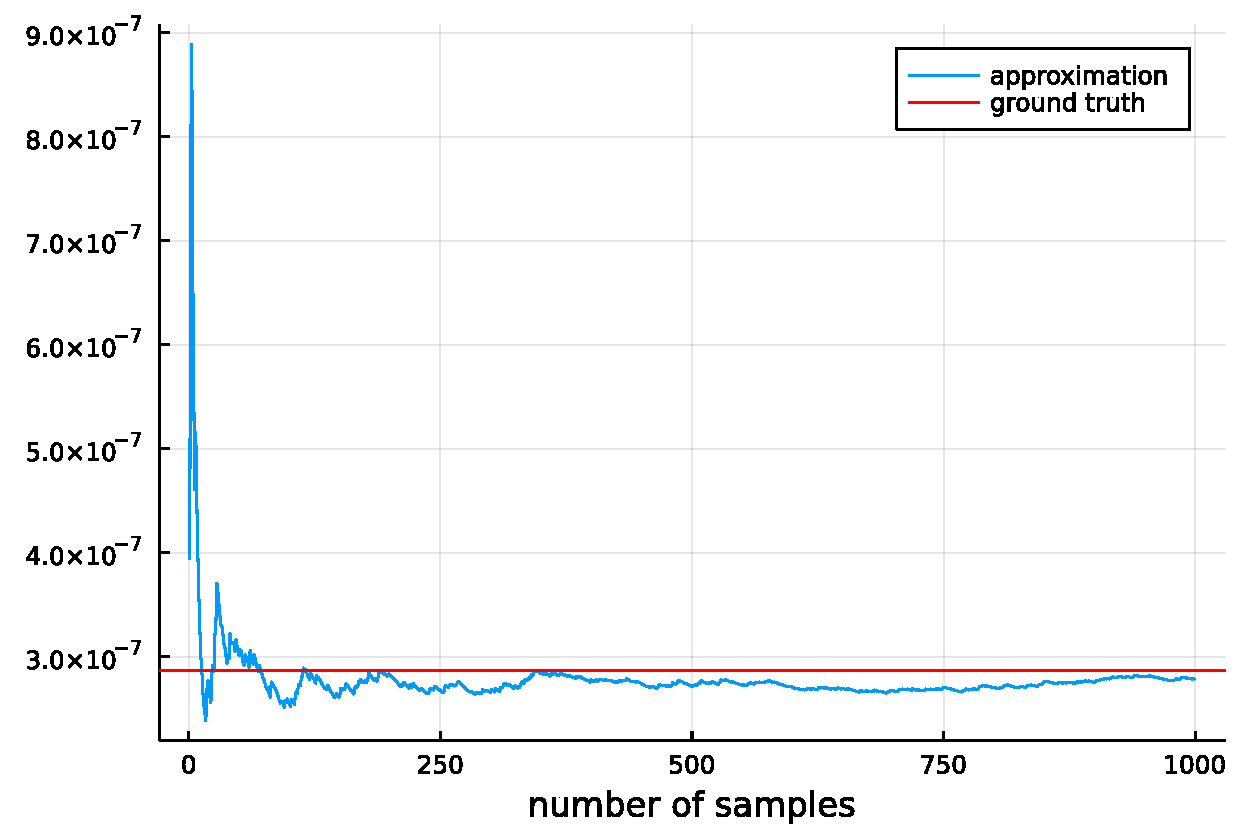
\includegraphics[width=0.75 \textwidth]{IS-tail-proba}
    \end{center}

    Python code is as follows.
    \begin{lstlisting}
      import numpy as np
      from numpy.random import default_rng
      import matplotlib.pyplot as plt
      from scipy.stats import norm

      n = 1000
      alpha = 5

      # compute the tail probability
      p = 1-norm.cdf(alpha)

      # sample from the importance distribution
      rng = default_rng()
      vals = rng.exponential(scale=1, size=n) + alpha

      # compute average
      def w(x):
      return 1/np.sqrt(2*np.pi)*np.exp(-x**2/2+x-alpha)

      Ihat = np.cumsum(w(vals))/ np.arange(1, n+1)

      # plot
      plt.plot(Ihat)
      plt.axhline(y=p, color="r")
      plt.xlabel("number of samples")
\end{lstlisting}
    
    And code in Julia is:
    \begin{lstlisting}
      using Distributions
      using Plots
      using Statistics

      # compute the tail probability
      phi(x) = cdf(Normal(0,1),x)
      alpha = 5
      p = (1-phi(alpha))

      # sample from the importance distribution
      n = 1000
      exprv = Exponential(1)
      x = rand(exprv, n).+alpha;

      # compute the approximation
      w(x) = 1/sqrt(2*pi)*exp(-x^2/2+x-alpha)
      #w(x) = pdf(Normal(0,1),x)/pdf(exprv, x-alpha);  

      Ihat = zeros(length(x));
      for k in 1:length(x)
         Ihat[k] = mean(w.(x[1:k]));
      end

      # plot
      plt=plot(Ihat, label="approximation");
      hline!([p], color=:red, label="ground truth")
      xlabel!("number of samples")
\end{lstlisting}
    
  \end{solution}
  
\end{exenumerate}


\ex{Monte Carlo integration and importance sampling}
\label{ex:monte-carlo-integration-and-importance-sampling}
A standard Cauchy distribution has the density function (pdf)
\begin{equation}
  \label{eq:cauchy-pdf}
  p(x) = \frac{1}{\pi}\frac{1}{1+x^2}
\end{equation}
with $x \in \mathbb{R}$. A friend would like to verify that $\int p(x)
dx =1$ but doesn't quite know how to solve the integral
analytically. They thus use importance sampling and approximate the integral as
\begin{equation}
  \int p(x) dx \approx \frac{1}{n} \sum_{i=1}^n \frac{p(x_i)}{q(x_i)} \quad \quad x_i \sim q
\end{equation}
where $q$ is the density of the auxiliary/importance
distribution. Your friend chooses a standard normal density for $q$
and produces the following figure:
\begin{center}
  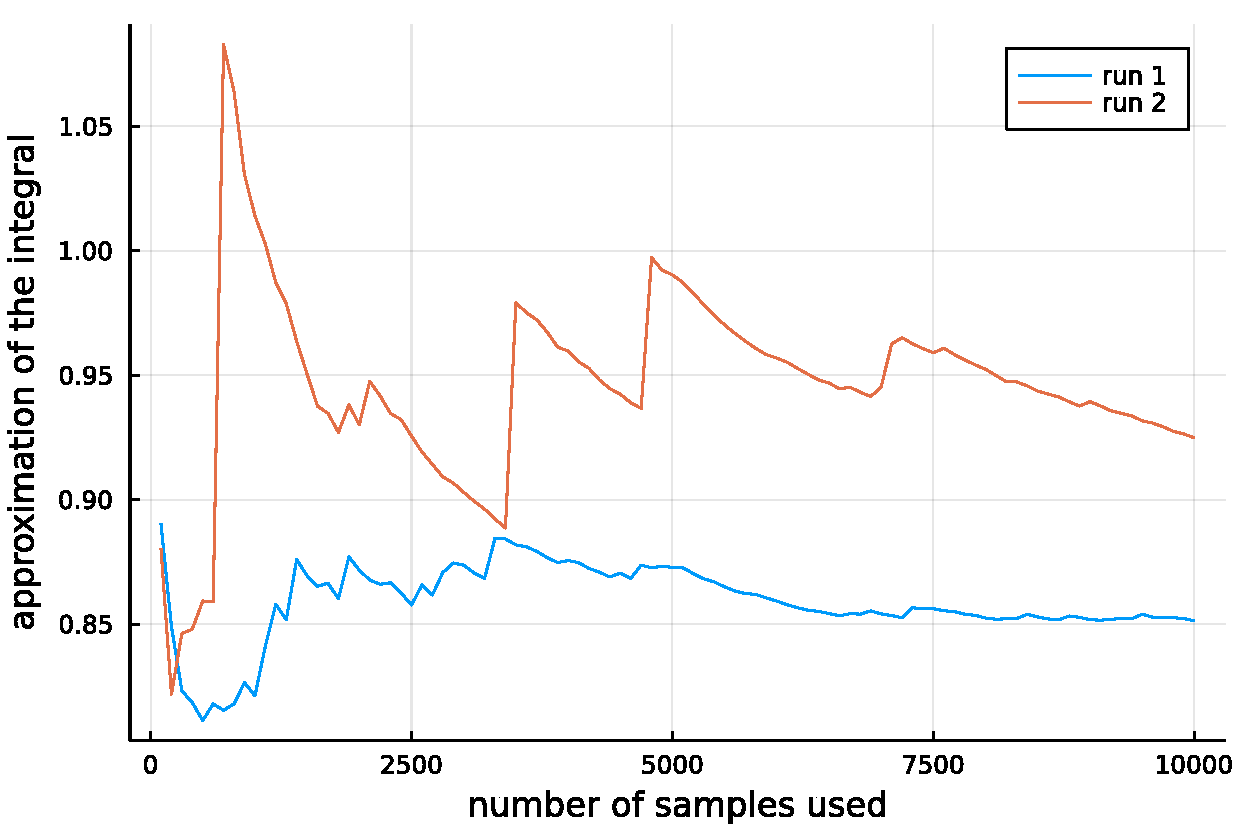
\includegraphics[width=0.65\textwidth]{traces_cauchy}
\end{center}
The figure shows two independent runs. In each run, your friend
computes the approximation with different sample sizes by subsequently
including more and more $x_i$ in the approximation, so that, for example, the
approximation with $n=2000$ shares the first 1000 samples with the
approximation that uses $n=1000$.

Your friend is puzzled that the two runs give rather different results
(which are not equal to one), and also that within each run, the
estimate very much depends on the sample size. Explain these findings.

\begin{solution}
  While the estimate $\hat{I}_n$
  \begin{equation}
    \hat{I}_n =  \frac{1}{n} \sum_{i=1}^n \frac{p(x_i)}{q(x_i)}
  \end{equation}
  is unbiased by construction, we have to check whether its second
  moment is finite. Otherwise, we have an invalid estimator that
  behaves erratically in practice. The ratio $w(x)$ between $p(x)$ and
  $q(x)$ equals
  \begin{align}
    w(x) & = \frac{p(x)}{q(x)}\\
    & = \frac{\frac{1}{\pi}\frac{1}{1+x^2}}{ \frac{1}{\sqrt{2\pi}}\exp(-x^2/2)}
  \end{align}
  which can be simplified to
  \begin{equation}
    w(x)  = \frac{\sqrt{2\pi}\exp(x^2/2)}{\pi(1+x^2)}.
  \end{equation}
  The second moment of $w(x)$ under $q(x)$ thus is
  \begin{align}
    \E_{q(x)}\left[w(x)^2\right] & = \int_{-\infty}^\infty \frac{2\pi}{\pi^2} \frac{\exp(x^2)}{(1+x^2)^2} q(x) dx\\
    & = \int_{-\infty}^\infty \frac{2\pi}{\pi^2} \frac{\exp(x^2)}{(1+x^2)^2} \frac{1}{\sqrt{2\pi}} \exp(-x^2/2) dx\\
    & \propto \int_{-\infty}^\infty \frac{\exp(x^2/2)}{(1+x^2)^2} dx
  \end{align}
  The exponential function grows more quickly than any polynomial so
  that the integral becomes arbitrarily large. Hence, the second
  moment (and the variance) of $\hat{I}_n$ is unbounded, which
  explains the erratic behaviour of the curves in the plot.

  A less formal but quicker way to see that, for this problem, a
  standard normal is a poor choice of an importance distribution is to
  note that its density decays more quickly than the Cauchy pdf in
  \eqref{eq:cauchy-pdf}, which means that the standard normal pdf is
  ``small'' when the Cauchy pdf is still ``large'' (see Figure
  \ref{fig:gauss-cauchy-logpdf}). This leads to large variance of the
  estimate. The overall conclusion is that the integral $\int p(x) dx$
  should not be approximated with importance sampling with a Gaussian
  importance distribution.

  \begin{figure}[h!]
    \centering
    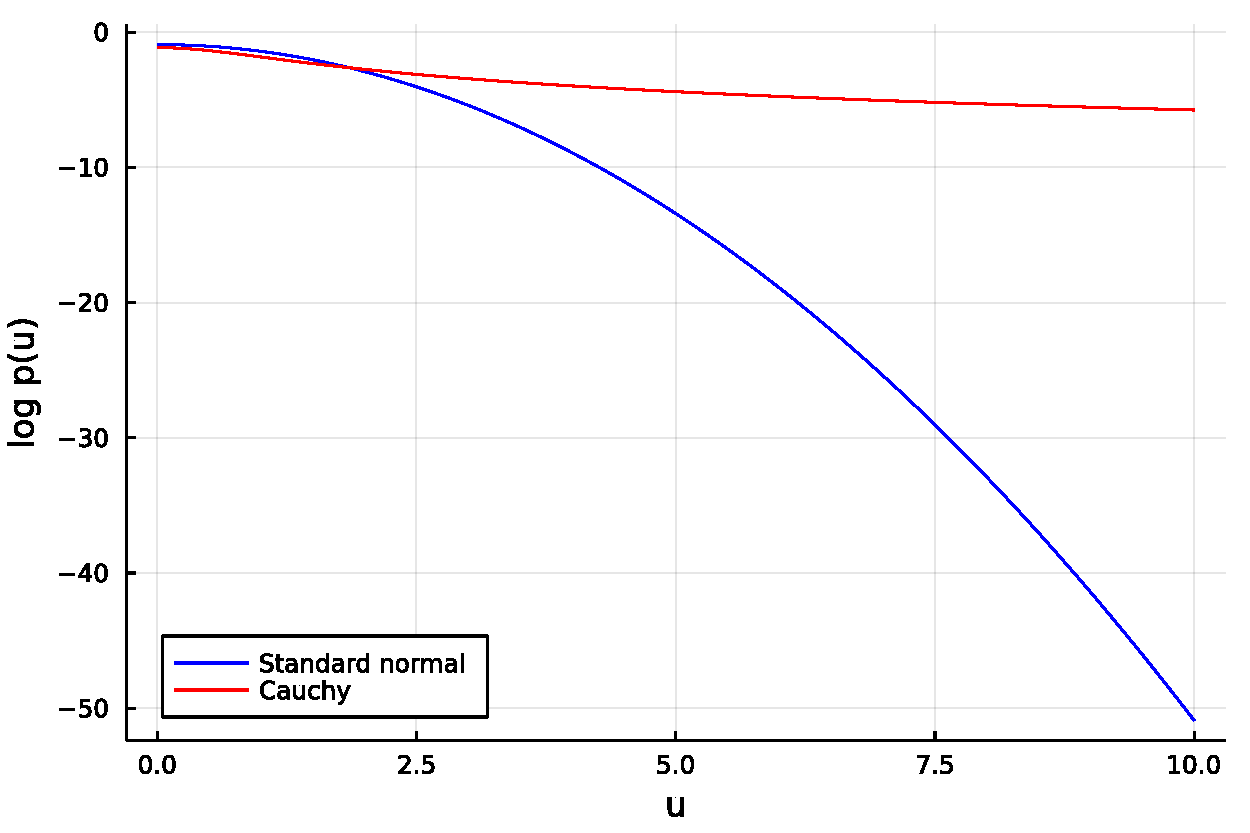
\includegraphics[width=0.6\textwidth]{gauss-cauchy-logpdf}
    \caption{\label{fig:gauss-cauchy-logpdf} Exercise
      \ref{ex:monte-carlo-integration-and-importance-sampling}. Comparison
      of the log pdf of a standard normal (blue) and the Cauchy random
      variable (red) for positive inputs. The Cauchy pdf has much
      heavier tails than a Gaussian so that the Gaussian pdf is
      already ``small'' when the Cauchy pdf is still ``large''.}
  \end{figure}
\end{solution}


\ex{Inverse transform sampling}
\label{ex:ex1}
The cumulative distribution function (cdf) $F_x(\alpha)$ of a (continuous or
discrete) random variable $x$ indicates the probability that $x$ takes
on values smaller or equal to $\alpha$,
\begin{equation}
  F_x(\alpha) = \Pr( x \le \alpha).
\end{equation}
For continuous random variables, the cdf is defined via the integral
\begin{equation}
  F_x(\alpha) = \int_{-\infty}^{\alpha} p_x(u) \ud u,
\end{equation}
where $p_x$ denotes the pdf of the random variable $x$ ($u$ is here a
dummy variable). Note that $F_x$ maps the domain of $x$ to the interval $[0,1]$. For simplicity, we here assume that $F_x$ is invertible.

For a continuous random variable $x$ with cdf $F_x$ show that the random variable $y = F_x(x)$ is uniformly distributed on $[0,1]$. 

Importantly, this implies that for a random variable $y$ which is
uniformly distributed on $[0,1]$, the transformed random variable
$F_x^{-1}(y)$ has cdf $F_x$. This gives rise to a method called
``inverse transform sampling'' to generate $n$ iid samples
of a random variable $x$ with cdf $F_x$.
%
Given a target cdf $F_x$, the method consists of:
\begin{itemize}
\item calculating the inverse $F_x^{-1}$
\item sampling $n$ iid random variables uniformly distributed on $[0,1]$: $y^{(i)} \sim \mathcal{U}(0,1)$, $i=1, \ldots, n$.
\item transforming each sample by $F_x^{-1}$: $x^{(i)} = F_x^{-1}(y^{(i)})$, $i=1, \ldots, n$.
\end{itemize}
By construction of the method, the $x^{(i)}$ are $n$ iid samples of $x$.
  
  \begin{solution}
    We start with the cumulative distribution function (cdf) $F_y$ for $y$,
    \begin{align}
      F_y(\beta) & = \Pr( y \le \beta).
    \end{align}
    Since $F_x(x)$ maps $x$ to $[0,1]$, $F_y(\beta)$ is zero for $\beta <0$ and one for $\beta>1$. We next consider $\beta \in [0,1]$.

   Let $\alpha$ be the value of $x$ that $F_x$ maps to $\beta$, i.e.\ $F_x(\alpha) = \beta$, which means $\alpha = F_x^{-1}(\beta)$. Since $F_x$ is a non-decreasing function, we have
    \begin{equation}
     F_y(\beta) = \Pr( y \le \beta) = \Pr( F_x(x) \le \beta) = \Pr(x \le F_x^{-1}(\beta)) = \Pr( x \le \alpha) = F_x(\alpha).
    \end{equation}
    Since $\alpha = F_x^{-1}(\beta)$ we obtain
    \begin{equation}
      F_y(\beta)  =  F_x( F_x^{-1}(\beta) ) = \beta
    \end{equation}
    The cdf $F_y$ is thus given by
    \begin{equation}
      F_y(\beta) = \begin{cases}
        0 & \text{if } \beta <0\\
        \beta & \text{if } \beta \in [0,1]\\
        1 & \text{if } \beta >1
      \end{cases}
    \end{equation}
    which is the cdf of a uniform random variable on $[0,1]$. Hence $y=F_x(x)$ is uniformly distributed on $[0,1]$.
    
  \end{solution}



\ex{Sampling from the exponential distribution}
The exponential distribution has the density
\begin{equation}
  p(x; \lambda) = \begin{cases} \lambda \exp(-\lambda x) & x \ge 0\\ 0
    & x<0,
  \end{cases}
  \end{equation}
where $\lambda$ is a parameter of the distribution. Use inverse transform sampling to generate $n$ iid samples from $p(x; \lambda)$.

\begin{solution}
  We first compute the cumulative distribution function.
  \begin{align}
    F_x(\alpha) & = \Pr(x\le \alpha)\\
    & = \int_0^\alpha  \lambda \exp(-\lambda x)\\
    & = -\exp(-\lambda)\big|_0^\alpha\\
    & = 1-\exp(-\lambda \alpha)
  \end{align}
  It's inverse is obtained by solving
  \begin{equation}
    y = 1-\exp(-\lambda x)
  \end{equation}
  for $x$, which gives:
  \begin{align}
    \exp(-\lambda x) &= 1-y\\
    -\lambda x &= \log(1-y)\\
    x &= \frac{-\log(1-y)}{\lambda}
  \end{align}
  To generate samples $x^{(i)}  \sim p(x; \lambda)$, we thus first sample $y^{(i)} \sim U(0,1)$, and then set
  \begin{equation}
    x^{(i)} = \frac{-\log(1-y^{(i)})}{\lambda}.
  \end{equation}
 
  Inverse transform sampling can be used to generate samples
  from many standard distributions. For example, it allows one
  to generate Gaussian random variables from uniformly
  distributed random variables. The method is called the
  Box-Muller transform, see
  e.g. \url{https://en.wikipedia.org/wiki/Box-Muller_transform}. How
  to generate the required samples from the uniform distribution is a
  research field on its own, see
  e.g. \url{https://en.wikipedia.org/wiki/Random_number_generation}
  and \citep[Chapter 3]{Owen2013}.

\end{solution}
  

\ex{Sampling from a Laplace distribution}
\label{ex:sampling-from-a-Laplace-distribution}
A Laplace random variable $x$ of mean zero and variance one has the density $p(x)$
\begin{equation}
  p(x) = \frac{1}{\sqrt{2}} \exp\left(-\sqrt{2}|x|\right) \quad \quad x \in \mathbb{R}.  
\end{equation}
Use inverse transform sampling to generate $n$ iid samples from $x$.

\begin{solution}
  The main task is to compute the cumulative distribution function (cdf) $F_x$ of $x$ and its inverse. The cdf is by definition
  \begin{align}
    F_x(\alpha) & = \int_{-\infty}^\alpha  \frac{1}{\sqrt{2}} \exp\left(-\sqrt{2}|u|\right) \ud u.
  \end{align}
  We first consider the case where $\alpha \le 0$. Since $-|u| = u$ for $u\le 0$, we have 
    \begin{align}
      F_x(\alpha) & = \int_{-\infty}^\alpha  \frac{1}{\sqrt{2}} \exp\left(\sqrt{2}u\right) \ud u   \\
      & = \frac{1}{2} \exp\left(\sqrt{2}u\right) \bigg |_{-\infty}^\alpha\\
      & =  \frac{1}{2} \exp\left(\sqrt{2} \alpha\right).
    \end{align}
  For $\alpha >0$, we have
   \begin{align}
     F_x(\alpha) & = \int_{-\infty}^\alpha  \frac{1}{\sqrt{2}} \exp\left(-\sqrt{2}|u|\right) \ud u   \\
     &= 1- \int_{\alpha}^\infty  \frac{1}{\sqrt{2}} \exp\left(-\sqrt{2}|u|\right) \ud u        
   \end{align}
  where we have used the fact that the pdf has to integrate to one. For values of $u>0$, $-|u| = -u$, so that
   \begin{align}
     F_x(\alpha) & = 1 - \int_{\alpha}^\infty  \frac{1}{\sqrt{2}} \exp\left(-\sqrt{2} u \right) \ud u  \\
     &= 1 + \frac{1}{2}  \exp\left(-\sqrt{2} u \right) \bigg |_{\alpha}^{\infty}\\
     &= 1 - \frac{1}{2}  \exp\left(-\sqrt{2} \alpha \right).
   \end{align}
  In total, for $\alpha \in \mathbb{R}$, we thus have
   \begin{equation}
     F_x(\alpha) = \begin{cases}
       \frac{1}{2} \exp\left(\sqrt{2} \alpha\right) & \text{if } \alpha \le 0\\
       1 - \frac{1}{2}  \exp\left(-\sqrt{2} \alpha\right) & \text{if } \alpha>0
     \end{cases}
   \end{equation}
  Figure \ref{fig:Fx} visualises $F_x(\alpha)$.
   \begin{figure}[h!]
     \centering
     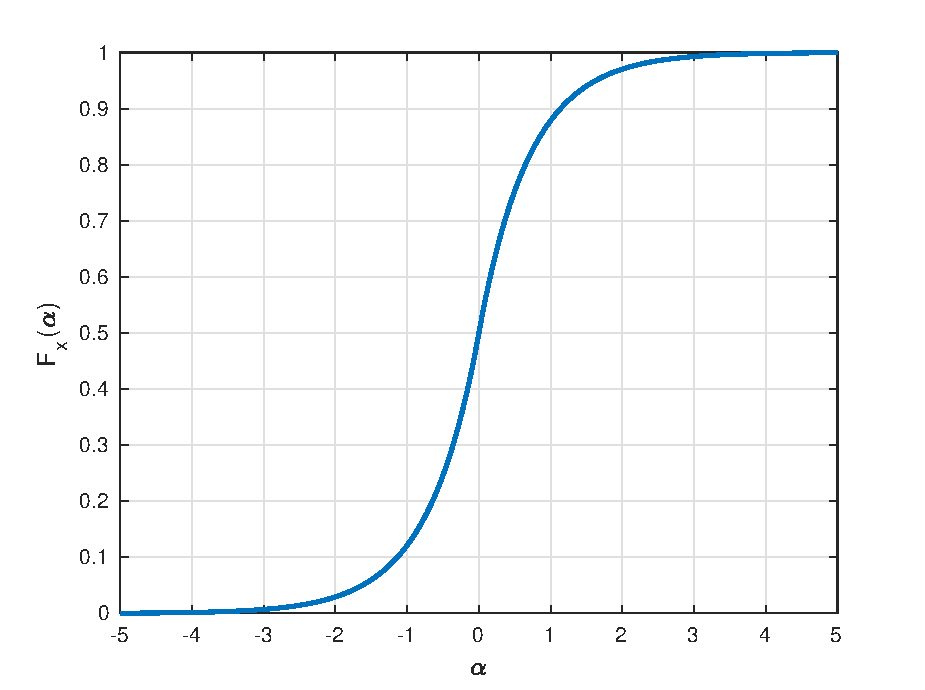
\includegraphics[width = 0.6 \textwidth]{cdf-laplace}
     \caption{\label{fig:Fx} The cumulative distribution function $F_x(\alpha)$ for a Laplace distributed random variable.}
   \end{figure}
   
  As the figure suggests, there is a unique inverse to $y = F_x(\alpha)$. For $y \le 1/2$, we have
   \begin{align}
     y & =  \frac{1}{2} \exp\left(\sqrt{2} \alpha\right)\\
     \log(2y) & = \sqrt{2} \alpha\\
     \alpha & = \frac{1}{\sqrt{2}} \log (2y)
   \end{align}
  For $y > 1/2$, we have
   \begin{align}
     y & =  1 - \frac{1}{2}  \exp\left(-\sqrt{2} \alpha \right)\\
     -y & =  -1 + \frac{1}{2}  \exp\left(-\sqrt{2} \alpha \right)\\
     1-y &= \frac{1}{2}  \exp\left(-\sqrt{2} \alpha \right) \\
     \log( 2-2y) & = -\sqrt{2} \alpha \\
     \alpha & = -\frac{1}{\sqrt{2}} \log(2-2y)
   \end{align}
  The function $y \mapsto g(y)$ that occurs in the logarithm in both cases is
   \begin{equation}
     g(y) = \begin{cases}
       2 y & \text{if } y\le \frac{1}{2}\\
       2-2y & \text{if } y> \frac{1}{2}
     \end{cases}.
   \end{equation}
  It is shown below and can be written more compactly as $g(y) = 1-2|y-1/2|$.
    \begin{figure}[h]
     \centering
     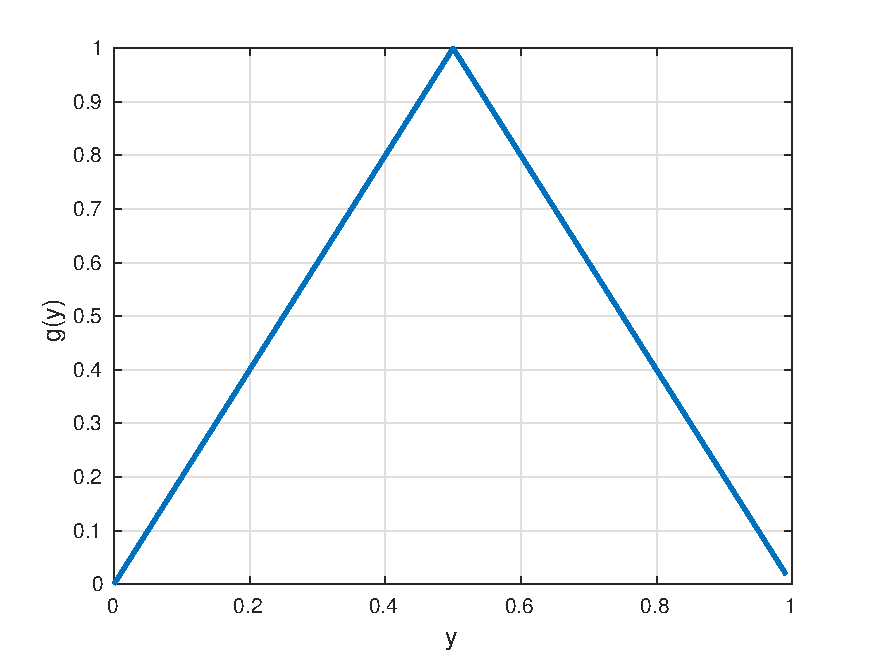
\includegraphics[width = 0.6 \textwidth]{g}
    \end{figure}

  We thus can write the inverse $F_x^{-1}(y)$ of the cdf $y=F_x(\alpha)$ as
    \begin{equation}
      F_x^{-1}(y) = -\text{sign}\left(y-\frac{1}{2}\right) \frac{1}{\sqrt{2}} \log\left[  1-2\big|y-\frac{1}{2}\big| \right].
    \end{equation}
  To generate $n$ iid samples from $x$, we first generate $n$
  iid samples $y^{(i)}$ that are uniformly distributed on $[0,1]$,
  and then compute for each $F_x^{-1}(y^{(i)})$. The properties of
  inverse transform sampling guarantee that the $x^{(i)}$,
    \begin{equation}
      x^{(i)} = F_x^{-1}(y^{(i)}),
    \end{equation}
  are independent and Laplace distributed.
  \end{solution}

\ex{Rejection sampling {\small \citep[based on][Exercise 2.8]{Robert2010}}}
\label{ex:rejection-sampling}
Most compute environments provide functions to sample from a standard
normal distribution. Popular algorithms include the Box-Muller
transform, see
e.g. \url{https://en.wikipedia.org/wiki/Box-Muller_transform}. We here
use rejection sampling to sample from a standard normal distribution
with density $p(x)$ using a Laplace distribution as our
proposal/auxiliary distribution.

The density $q(x)$ of a zero-mean Laplace distribution with variance
$2b^2$ is
\begin{equation}
  q(x;b) = \frac{1}{2b}\exp\left(-\frac{|x|}{b}\right).
\end{equation}
We can sample from it by sampling a Laplace variable with variance 1
as in Exercise \ref{ex:sampling-from-a-Laplace-distribution} and then
scaling the sample by $\sqrt{2}b$.

Rejection sampling then repeats the following steps:
\begin{itemize}
  \item Generate $x \sim q(x; b)$
  \item Accept $x$ with probability $f(x) = \frac{1}{M}
    \frac{p(x)}{q(x)}$, i.e. generate $u \sim U(0,1)$ and accept $x$
    if $u \le f(x)$.
\end{itemize}

\begin{exenumerate}
\item Compute the ratio $M(b) = \max_x \frac{p(x)}{q(x; b)}$.
  \begin{solution}
    By the definitions of the pdf $p(x)$ of a standard normal and the pdf $q(x; b)$ of the Laplace distribution, we have
    \begin{align}
      \frac{p(x)}{q(x;b)} &= \frac{ \frac{1}{\sqrt{2\pi}} \exp(-x^2/2)}{\frac{1}{2b}\exp(-|x|/b)}\\
          & = \frac{2b}{\sqrt{2\pi}} \exp(-x^2/2 + |x|/b)
    \end{align}
    The ratio is symmetric in $x$. Moreover, since the exponential
    function is strictly increasing, we can find the maximiser of
    $-x^2/2+x/b$ for $x\ge 0$ to determine the maximiser of
    $M(b)$. With $g(x) = -x^2/2+x/b$, we have
    \begin{align}
      g'(x) &= -x + 1/b\\
      g''(x) &= -1
    \end{align}
    The critical point (for which the first derivative is zero) is $x = 1/b$ and since the second derivative is negative for all $x$, the point is a maximum. The maximal ratio $M(b)$ thus is
    \begin{align}
      M(b)  & = \frac{2b}{\sqrt{2\pi}} \exp\left(-x^2/2 + |x|/b\right)\Big|_{x=1/b}\\
      & = \frac{2b}{\sqrt{2\pi}} \exp\left(-1/(2b^2) + 1/b^2\right)\\
      & = \frac{2b}{\sqrt{2\pi}} \exp\left(1/(2b^2)\right)
    \end{align}
  \end{solution}

\item How should you choose $b$ to maximise the probability of acceptance?

  \begin{solution}
    The probability of acceptance is $1/M$. Hence to maximise it, we
    have to choose $b$ such that $M(b)$ is minimal. We compute the derivatives
    \begin{align}
      M'(b) & = \frac{2}{\sqrt{2\pi}} \exp(1/(2b^2)) - \frac{2b}{\sqrt{2\pi}} \exp(1/(2b^2)) b^{-3}\\
      & = \frac{2}{\sqrt{2\pi}} \exp(1/(2b^2)) - \frac{2}{\sqrt{2\pi}} \exp(1/(2b^2)) b^{-2}\\
      & = \frac{2}{\sqrt{2\pi}} \exp(1/(2b^2))(1-b^{-2})\\
      M''(b) & = -b^{-3}\frac{2}{\sqrt{2\pi}} \exp(1/(2b^2))(1-b^{-2})+2b^{-3}\frac{2}{\sqrt{2\pi}} \exp(1/(2b^2))\\
    \end{align}
    Setting the first derivative to zero gives
    \begin{align}
      \frac{2}{\sqrt{2\pi}} \exp(1/(2b^2)) &= \frac{2}{\sqrt{2\pi}} \exp(1/(2b^2)) b^{-2}\\
      1 & = b^{-2}
    \end{align}
    Hence the optimal $b=1$. The second derivative at $b=1$ is
    \begin{align}
      M''(1) & = 2 \frac{2}{\sqrt{2\pi}} \exp(1/2)
    \end{align}
    which is positive so that the $b=1$ is a minimum. The smallest value of $M$ thus is
    \begin{align}
      M(1) & =  \frac{2b}{\sqrt{2\pi}} \exp(1/(2b^2))\Big |_{b=1} \\
      & =  \frac{2}{\sqrt{2\pi}} \exp(1/2)\\
      & =  \sqrt{\frac{2 e}{\pi}}
    \end{align}
    where $e=\exp(1)$. The maximal acceptance probability thus is
    \begin{align}
      \frac{1}{\min_b M(b)} & = \sqrt{\frac{\pi}{2e}}\\
      & \approx 0.76
    \end{align}
    This means for each sample $x$ generated from $q(x; 1)$, there is
    chance of $0.76$ that it gets accepted. In other words, for each
    accepted sample, we need to generate $1/0.76 = 1.32$ samples from
    $q(x; 1)$.

    The variance of the Laplace distribution for $b=1$ equals 2. Hence
    the variance of the auxiliary distribution is larger (twice as
    large) as the variance of the distribution we would like to sample from. 
  \end{solution}
\item Assume you sample from $p(x_1, \ldots, x_d) = \prod_{i=1}^d
  p(x_i)$ using $q(x_1, \ldots, x_d) = \prod_{i=1}^d q(x_i; b)$ as
  auxiliary distribution without exploiting any independencies. How
  does the acceptance probability scale as a function of $d$? You may
  denote the acceptance probability in case of $d=1$ by $A$.

  \begin{solution}
    We have to determine the maximal ratio
    \begin{equation}
      M_d = \max_{x_1, \ldots, x_d} \frac{p(x_1, \ldots, x_d)}{q(x_1, \ldots, x_d)}
    \end{equation}
    Plugging-in the factorisation gives
    \begin{align}
      M_d &= \max_{x_1, \ldots, x_d} \prod_{i=1}^d \frac{p(x_i)}{q(x_i)}\\
      & = \prod_{i=1}^d \underbrace{\max_{x_i} \frac{p(x_i)}{q(x_i)}}_{M_1 = 1/A}\\
      & = \prod_{i=1}^d \frac{1}{A}\\
      & = \frac{1}{A^d}
    \end{align}
    Hence, the acceptance probability is
    \begin{equation}
      \frac{1}{M_d} = A^d
    \end{equation}
    Note that $A\le 1$ since it is a probability. This means that, unless $A=1$, we
    have an acceptance probability that decays exponentially in the
    number of dimensions if the target and auxiliary distributions
    factorise and we do not exploit the independencies.
  \end{solution}
\end{exenumerate}


\ex{Sampling from a restricted Boltzmann machine}

The restricted Boltzmann machine (RBM) is a model for binary variables
$\v =(v_1, \ldots, v_n)^\top$ and $\h=(h_1, \ldots, h_m)^\top$ which
asserts that the joint distribution of $(\v,\h)$ can be described by
the probability mass function
\begin{equation}
  p(\v,\h) \propto \exp\left( \v^\top \W \h + \a^\top\v + \b^\top\h \right),
\end{equation}
where $\W$ is a $n \times m$ matrix, and $\a$ and $\b$ vectors of size
$n$ and $m$, respectively. Both the $v_i$ and $h_i$ take
values in $\{0,1\}$. The $v_i$ are called the ``visibles'' variables
since they are assumed to be observed while the $h_i$ are the hidden
variables since it is assumed that we cannot measure them.

Explain how to use Gibbs sampling to generate samples from the
marginal $p(\v)$,
  \begin{equation}
    p(\v) = \frac{\sum_{\h}  \exp\left( \v^\top \W \h + \a^\top\v + \b^\top\h \right)}{\sum_{\h, \v}  \exp\left( \v^\top \W \h + \a^\top\v + \b^\top\h \right)},
  \end{equation}
for any given values of $\W$, $\a$, and $\b$.

\emph{Hint:} You may use that
\begin{align}
  p(\h | \v) &= \prod_{i=1}^m p(h_i | \v), &  p(h_i=1 | \v) & =  \frac{1}{ 1+  \exp\left(- \sum_j v_j W_{ji} - b_i \right)}, \\
  p(\v | \h) &= \prod_{i=1}^n p(v_i | \h), &  p(v_i = 1 | \h) &= \frac{1}{1+\exp\left(-\sum_j W_{ij} h_j-a_i\right)}.
\end{align}


\begin{solution}
In order to generate samples $\v^{(k)}$ from $p(\v)$ we generate
samples $(\v^{(k)}, \h^{(k)})$ from $p(\v, \h)$ and then ignore the
$\h^{(k)}$.

Gibbs sampling is a MCMC method to produce a sequence of samples
$\x^{(1)}, \x^{(2)}, \x^{(3)}, \ldots$ that follow a pdf/pmf $p(\x)$
(if the chain is run long enough). Assuming that $\x$ is
$d$-dimensional, we generate the next sample $\x^{(k+1)}$ in the
sequence from the previous sample $\x^{(k)}$ by:
\begin{enumerate}
  \item picking (randomly) an index $i \in \{1, \ldots, d \}$
  \item sampling $x_i^{(k+1)}$ from $p(x_i \mid \x^{(k)}_{\backslash
    i})$ where $\x^{(k)}_{\backslash i}$ is vector $\x$ with $x_i$
    removed, i.e. $\x^{(k)}_{\backslash i}
    =({x}_1^{(k)},\ldots,{x}_{i-1}^{(k)},{x}_{i+1}^{(k)},\ldots,{x}_d^{(k)})$
  \item setting $\x^{(k+1)} =({x}_1^{(k)},\ldots,{x}_{i-1}^{(k)},x_i^{(k+1)},{x}_{i+1}^{(k)},\ldots,{x}_d^{(k)})$.
\end{enumerate}
For the RBM, the tuple $(\h,\v)$ corresponds to $\x$ so that a $x_i$
in the above steps can either be a hidden variable or a visible. Hence
\begin{equation}
  p(x_i \mid \x_{\backslash i}) = \begin{cases}
    p(h_i \mid \h_{\backslash i}, \v) & \text{if $x_i$ is a hidden variable $h_i$}\\
    p(v_i \mid \v_{\backslash i}, \h) & \text{if $x_i$ is a visible variable $v_i$}
  \end{cases}
\end{equation}
($\h_{\backslash i}$ denotes the vector $\h$ with element $h_i$
removed, and equivalently for $\v_{\backslash i}$)

To compute the conditionals on the right hand side, we use the hint:
\begin{align}
  p(\h | \v) &= \prod_{i=1}^m p(h_i | \v), &  p(h_i=1 | \v) & =  \frac{1}{ 1+  \exp\left(- \sum_j v_j W_{ji} - b_i \right)}, \\
  p(\v | \h) &= \prod_{i=1}^n p(v_i | \h), &  p(v_i = 1 | \h) &= \frac{1}{1+\exp\left(-\sum_j W_{ij} h_j-a_i\right)}.
\end{align}
Given the independencies between the hiddens given the visibles and vice versa, we have
\begin{align}
  p(h_i \mid \h_{\backslash i}, \v) & = p(h_i \mid \v) &   p(v_i \mid \v_{\backslash i}, \h) & = p(v_i \mid \h)
\end{align}
so that the expressions for $p(h_i=1 | \v)$ and $p(v_i = 1 | \h)$ allow us to implement the Gibbs sampler.

Given the independencies, it makes further sense to sample the $\h$
and $\v$ variables in blocks: first we sample all the $h_i$ given
$\v$, and then all the $v_i$ given the $\h$ (or vice versa). This is
also known as block Gibbs sampling.

In summary, given a sample $(\h^{(k)},\v^{(k)})$, we thus generate the next sample
$(\h^{(k+1)},\v^{(k+1)})$ in the sequence as follows:
\begin{itemize}
\item For all $h_i$, $i=1, \ldots, m$:
  \begin{itemize}
  \item compute $p^h_i = p(h_i=1 | \v^{(k)})$
  \item sample $u_i$ from a uniform distribution on $[0,1]$ and set $h^{(k+1)}_i$ to 1 if $u_i \le p^h_i$.
  \end{itemize}
\item For all $v_i$, $i=1, \ldots, n$:
  \begin{itemize}
  \item compute $p^v_i = p(v_i=1 | \h^{(k+1)})$
  \item sample $u_i$ from a uniform distribution on $[0,1]$ and set $v^{(k+1)}_i$ to 1 if $u_i \le p^v_i$.
  \end{itemize}
\end{itemize}
As final step, after sampling $S$ pairs $(\h^{(k)},\v^{(k)})$, $k=1,
\ldots, S$, the set of visibles $\v^{(k)}$ form samples from the
marginal $p(\v)$.
\end{solution}



\ex{Basic Markov chain Monte Carlo inference} \label{q:basic-mcmc}
This exercise is on sampling and approximate inference by Markov
chain Monte Carlo (MCMC). MCMC can be used to obtain
samples from a probability distribution, e.g. a posterior
distribution. The samples approximately represent the distribution, as
illustrated in Figure~\ref{fig:mcmc_approx}, and can be used to
approximate expectations.

We denote the density of a zero mean Gaussian with variance $\sigma^2$ by
$\normal(x; \mu, \sigma^2)$, i.e.\
\begin{equation}
  \normal(x; \mu, \sigma^2) = \frac{1}{\sqrt{2\pi \sigma^2}}\exp\left(-\frac{(x-\mu)^2}{2\sigma^2}\right)
\end{equation}

\begin{figure}[!h]
	\centering
	\subfloat[True density]{
	  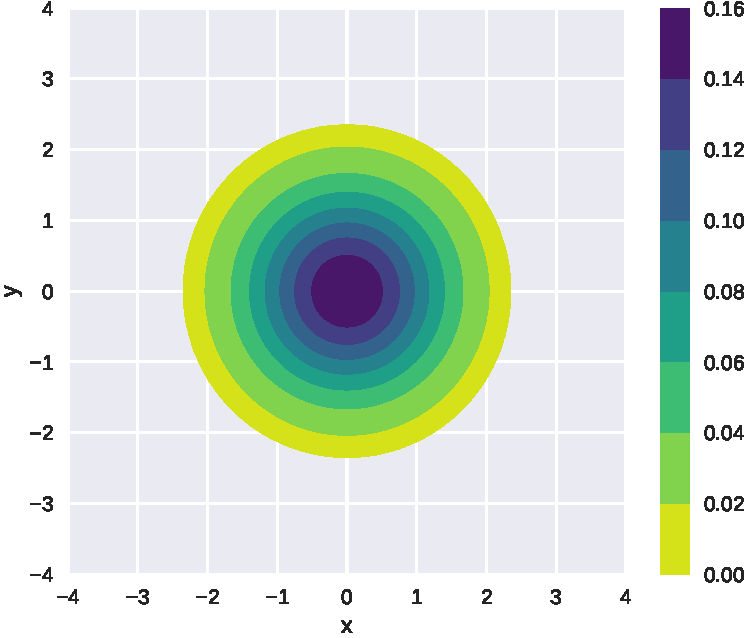
\includegraphics[width=0.45\textwidth]{density}
	  \label{sfig:density}}
	\subfloat[Density represented by $10,000$ samples.]{
	  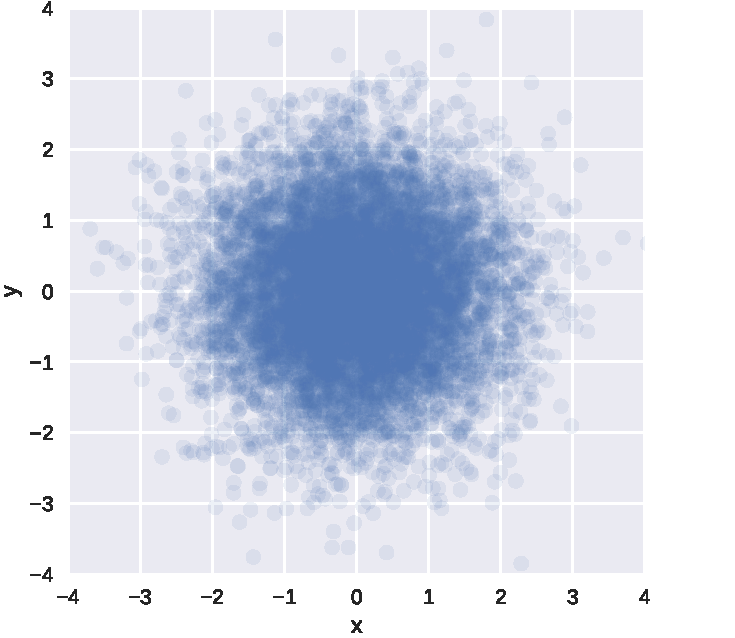
\includegraphics[width=0.45\textwidth]{scatter}
	  \label{sfig:scatter}
        }
	\caption{Density and samples from $p(x,y) = \normal(x; 0,1)\normal(y;0,1)$.}
	\label{fig:mcmc_approx}
\end{figure}

Consider a vector of $d$ random variables $\thetab = (\theta_1, \dots, \theta_d)$ and some observed data $\data$.
%
In many cases, we are interested in computing expectations under
the posterior distribution $p(\thetab \mid \data)$, e.g.\
\begin{equation}
  \E_{p(\thetab \mid \data)}\left[g(\thetab)\right] = \int g(\thetab) p(\thetab \mid \data) \mathrm{d} \thetab
\end{equation}
for some function $g(\thetab)$. If $d$ is small, e.g.\ $d \le3$, deterministic
numerical methods can be used to approximate the integral to high accuracy, see
e.g.\ \url{https://en.wikipedia.org/wiki/Numerical_integration}. But for higher
dimensions, these methods are generally not applicable any more. The
expectation, however, can be approximated as a sample average if we have samples
$\thetab^{(i)}$ from $p(\thetab \mid \data)$:
\begin{equation}
\E_{p(\thetab \mid \data)}\left[g(\thetab)\right] \approx \frac{1}{S}\sum_{i=1}^{S} g(\thetab^{(i)})
\end{equation}
Note that in MCMC methods, the samples $\thetab^{(1)}, \ldots, \thetab^{(S)}$ used in the above
approximation are typically not statistically independent.

Metropolis-Hastings is an MCMC algorithm that generates samples from a
distribution $p(\thetab)$, where $p(\thetab)$ can be any distribution
on the parameters (and not only posteriors). The algorithm is iterative
and at iteration $t$, it uses:
\begin{itemize}
\item a proposal distribution $q(\thetab; \thetab^{(t)})$, parametrised by the
	current state of the Markov chain, i.e.\ $\thetab^{(t)}$;
\item a function $p^*(\thetab)$, which is proportional to $p(\thetab)$. In other
  words, $p^*(\thetab)$ is unnormalised\footnote{We here follow the notation of \citet{Barber2012}; $\tilde{p}$ or $\phi$ are often to denote unnormalised models too.} and the normalised density
  $p(\thetab)$ is
  \begin{equation} p(\thetab) = \frac{p^*(\thetab)}{\int p^*(\thetab) \mathrm{d}\thetab}.
  \end{equation}
\end{itemize} 
For all tasks in this exercise, we work with a Gaussian proposal distribution
$q(\thetab; \thetab^{(t)})$, whose mean is the previous sample in the Markov
chain, and whose variance is $\epsilon^2$. That is, at iteration $t$ of our
Metropolis-Hastings algorithm,
\begin{equation}
  q(\thetab; \thetab^{(t-1)}) = \prod_{k=1}^d\normal(\theta_k; \theta_k^{(t-1)}, \epsilon^2).
  \label{eq:gauss-prop}
\end{equation}
When used with this proposal distribution, the algorithm is
called Random Walk Metropolis-Hastings algorithm.
%


\begin{exenumerate}
\item Read Section 27.4 of \citet{Barber2012} to familiarise yourself with the Metropolis-Hastings algorithm.

\item\label{qpt:mh} Write a function \lstinline|mh| implementing the
  Metropolis Hasting algorithm, as given in Algorithm 27.3 in
\citet{Barber2012}, using the Gaussian proposal distribution in \eqref{eq:gauss-prop} above. The
  function should take as arguments
\begin{itemize}
	\item \lstinline{p_star}: a function on $\thetab$ that is proportional to the density of interest $p(\thetab)$;
	\item \lstinline{param_init}: the initial sample --- a value for $\thetab$ from where the Markov chain starts;
	\item \lstinline{num_samples}: the number $S$ of samples to generate;
	\item \lstinline{vari}: the variance $\epsilon^2$ for the Gaussian proposal distribution $q$;
\end{itemize}
and return $[\thetab^{(1)}, \dots, \thetab^{(S)}]$ --- a list of $S$ samples from $p(\thetab) \propto p^*(\thetab)$. For example:
\begin{lstlisting}
  def mh(p_star, param_init, num_samples=5000, vari=1.0):
      # your code here
      return samples
\end{lstlisting}



\begin{solution}


  Below is a Python implementation.
\begin{lstlisting}
def mh(p_star, param_init, num_samples=5000, vari=1.0):
   x = []

   x_current = param_init
   for n in range(num_samples):

     # proposal
     x_proposed = multivariate_normal.rvs(mean=x_current, cov=vari)

     # MH step
     a = multivariate_normal.pdf(x_current, mean=x_proposed, cov=vari) * p_star(x_proposed)
     a = a / (multivariate_normal.pdf(x_proposed, mean=x_current, cov=vari) * p_star(x_current))

     # accept or not 
     if a >= 1:
       x_next = np.copy(x_proposed)
     elif uniform.rvs(0, 1) < a:
       x_next = np.copy(x_proposed)
     else:
       x_next = np.copy(x_current)

     # keep record
     x.append(x_next)
     x_current = x_next
	
   return x
\end{lstlisting}
%
As we are using a symmetrical proposal distribution, $q(\thetab \mid \thetab^*) = q(\thetab^* \mid \thetab)$, and one could simplify the algorithm by having $a = \frac{p^*(\thetab^*)}{p^*(\thetab)}$, where $\thetab$ is the current sample and $\thetab^*$ is the proposed sample.

In practice, it is desirable to implement the function in the log domain, to avoid numerical problems. That is, instead of $p^*$, \lstinline|mh| will accept as an argument $\log p^*$, and $a$ will be calculated as: 
$$a = (\log q(\thetab \mid \thetab^*) + \log p^*(\thetab^*)) - (\log q(\thetab^* \mid \thetab) + \log p^*(\thetab))$$
\end{solution}

\item \label{qpt:mh_test} Test your algorithm by sampling $5,000$
  samples from $p(x, y) = \normal(x; 0, 1)\normal(y; 0,
  1)$. Initialise at $(x=0, y=0)$ and use $\epsilon^2=1$.
%
Generate a scatter plot of the obtained samples. The plot should be
similar to Figure~\ref{sfig:scatter}. Highlight the first 20 samples
only. Do these 20 samples alone adequately approximate the true
density?

Sample another $5,000$ points from $p(x, y) = \normal(x; 0,
1)\normal(y; 0, 1)$ using \lstinline|mh| with $\epsilon^2=1$, but this
time initialise at $(x=7,y=7)$. Generate a scatter plot of the drawn
samples and highlight the first 20 samples. If everything went as
expected, your plot probably shows a ``trail'' of samples, starting at
$(x=7, y=7)$ and slowly approaching the region of space where most of
the probability mass is.


\begin{solution}

  \begin{figure}[!h]
    \captionsetup{type=figure}% tell subfig package that this is a figure
    \centering
    \subfloat[\label{sfig:00} Starting the chain at $(0,0)$.]{
      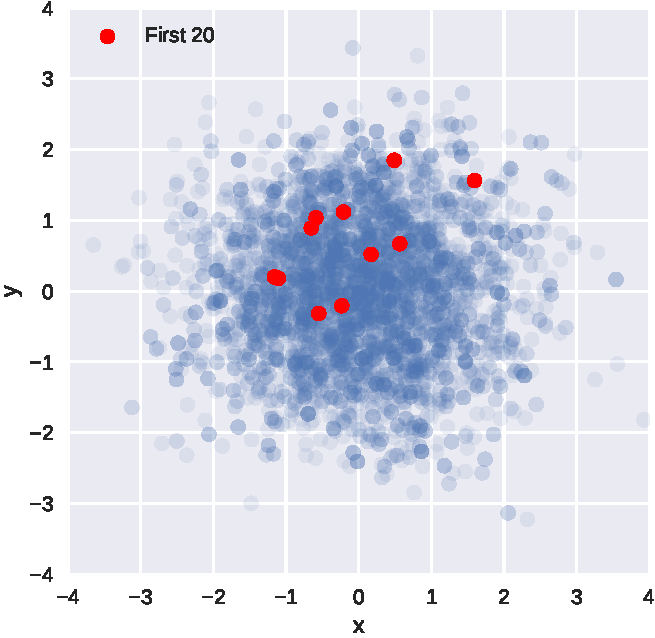
\includegraphics[width=0.45\textwidth]{00_warmup}}
    \subfloat[\label{sfig:77}Starting the chain at $(7,7)$]{
      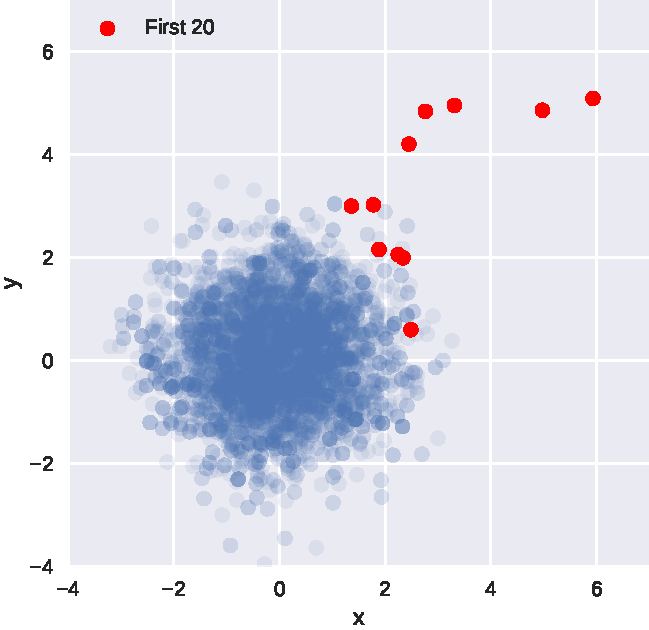
\includegraphics[width=0.45\textwidth]{77_warmup}}
    \caption{\label{fig:initial} $5,000$ samples from $\normal(x; 0, 1)\normal(y; 0, 1)$ (blue), with the first $20$ samples highlighted (red). Drawn using Metropolis-Hastings with different starting points.}
  \end{figure}


Figure~\ref{fig:initial} shows the two scatter plots of draws from $\normal(x; 0, 1)\normal(y; 0, 1)$:
\begin{itemize}
	\item Figure~\ref{sfig:00} highlights the first 20 samples
          obtained by the chain when starting at $(x=0, y=0)$. They
          appear to be representative samples from the distribution,
          however, they are not enough to approximate the distribution
          on their own. This would mean that a sample average computed
          with 20 samples only would have high variance, i.e. its
          value would depend strongly on the values of the 20 samples
          used to compute the average.
	\item Figure~\ref{sfig:77} highlights the first 20 samples
          obtained by the chain when starting at $(x=7, y=7)$. One can
          clearly see the ``burn-in'' tail which slowly approaches the
          region where most of the probability mass is.
\end{itemize}


\end{solution}

\item In practice, we don't know where the distribution we wish to
  sample from has high density, so we typically initialise the Markov
  Chain somewhat arbitrarily, or at the maximum a-posterior (MAP) sample if
  available. The samples obtained in the beginning of the chain are
  typically discarded, as they are not considered to be representative
  of the target distribution. This initial period between
  initialisation and starting to collect samples is called
  ``warm-up'', or also ``burn-in''.

Extended your function \lstinline|mh| to include an additional warm-up
argument $W$, which specifies the number of MCMC steps taken before
starting to collect samples. Your function should still return a list
of $S$ samples as in \ref{qpt:mh}.

\begin{solution}

We can extend the \lstinline|mh| function with a warm-up argument by, for example, iterating for \lstinline|num_samples + warmup|
steps, and start recording samples only after the warm-up period:
\begin{lstlisting}
def mh(p_star, param_init, num_samples=5000, vari=1.0, warmup=0):
	x = []
	x_current = param_init
	for n in range(num_samples+warmup):
		...  # body same as before
	
		if n >= warmup: x.append(x_next)
		x_current = x_next
	
	return x
\end{lstlisting}
\end{solution}

\end{exenumerate}


\ex{Bayesian Poisson regression}\label{q:poisson-reg}
  Consider a Bayesian Poisson regression
  model, where outputs $y_n$ are generated from a Poisson distribution
  of rate $\exp(\alpha x_n + \beta)$, where the $x_n$ are the inputs (covariates), and $\alpha$ and $\beta$ the parameters of the regression model for which we assume a broad Gaussian prior:
  \begin{align}
    \alpha &\sim \normal(\alpha; 0, 100) \\
    \beta &\sim \normal(\beta; 0, 100)\\
    y_n &\sim \mathrm{Poisson}(y_n; \exp(\alpha x_n + \beta)) \quad \text{for } n = 1, \dots, N 
\end{align}
$\mathrm{Poisson}(y ;\lambda)$ denotes the probability mass
function of a Poisson random variable with rate $\lambda$,
\begin{equation}
  \mathrm{Poisson}(y; \lambda) = \frac{\lambda^y}{y!}\exp(-\lambda), \quad \quad y \in \{0, 1, 2, \ldots\}, \quad \lambda>0
\end{equation}
Consider $\data = \{(x_n, y_n)\}_{n=1}^N$ where $N=5$ and
\begin{align}
(x_1, \ldots, x_5) &= (-0.50519053, -0.17185719,  0.16147614,  0.49480947,  0.81509851)\\
  (y_1, \ldots, y_5) &= (1, 0, 2, 1, 2)
\end{align}

We are interested in computing the posterior density of the parameters
$(\alpha, \beta)$ given the data $\data$ above.

\begin{exenumerate}

\item Derive an expression for the unnormalised posterior density of
  $\alpha$ and $\beta$ given $\data$, i.e. a function $p^*$ of the
  parameters $\alpha$ and $\beta$ that is proportional to the
  posterior density $p(\alpha, \beta\mid \data)$, and which can thus
  be used as target density in the Metropolis Hastings algorithm.
  
  \begin{solution}
    By the product rule, the joint distribution described by the
    model, with $\data$ plugged in, is proportional to the posterior
    and hence can be taken as $p^*$:
    \begin{align}
      p^*(\alpha, \beta) &= p(\alpha, \beta, \{(x_n,y_n)\}_{n=1}^N ) \\ 
      &= \normal(\alpha; 0, 100)\normal(\beta; 0, 100)\prod_{n=1}^{N}\mathrm{Poisson}(y_n \mid \text{exp}(\alpha x_n + \beta))
    \end{align}
  \end{solution}
  
\item Implement the derived unnormalised posterior density $p^*$. If
  your coding environment provides an implementation of the above
  Poisson pmf, you may use it directly rather than implementing the
  pmf yourself.

  Use the Metropolis Hastings algorithm from Question
  \ref{q:basic-mcmc}\ref{qpt:mh_test} to draw $5,000$ samples from the
  posterior density $p(\alpha, \beta\mid \data)$. Set the
  hyperparameters of the Metropolis-Hastings algorithm to:
    \begin{itemize}
    \item \lstinline{param_init} $=(\alpha_{\mathrm{init}},\beta_{\mathrm{init}}) = (0,0)$,
    \item \lstinline{vari} $= 1$, and 
    \item number of warm-up steps $W = 1000$.
    \end{itemize}
    
    Plot the drawn samples with x-axis $\alpha$ and y-axis $\beta$ and report the posterior mean of $\alpha$ and $\beta$, as well as their correlation coefficient under the posterior.

    \begin{solution}
      A Python implementation is:
      
      \begin{lstlisting}
import numpy as np
from scipy.stats import multivariate_normal, norm, poisson, uniform

xx1 = np.array([-0.5051905265552105, -0.17185719322187715, 0.16147614011145617, 0.49480947344478954, 0.8150985069051909])
yy1 = np.array([1, 0, 2, 1, 2])
N1 = len(xx1)

def poisson_regression(params):
    a = params[0]
    b = params[1]
    # mean zero, standard deviation 10 == variance 100
    p = norm.pdf(a, loc=0, scale=10) * norm.pdf(b, loc=0, scale=10) 
    for n in range(N1):
        p = p * poisson.pmf(yy1[n], np.exp(a * xx1[n] + b)) 

    return p

# sample
S = 5000
samples = np.array(mh(poisson_regression, np.array([0, 0]), num_samples=S, vari=1.0, warmup=1000))
\end{lstlisting}

A scatter plot showing $5,000$ samples from the posterior is shown on
Figure~\ref{fig:easy}. The posterior mean of $\alpha$ is 0.84, the
posterior mean of $\beta$ is -0.2, and posterior correlation
coefficient is -0.63. Note that the numerical values are sample-specific.
\begin{figure}
  \centering
  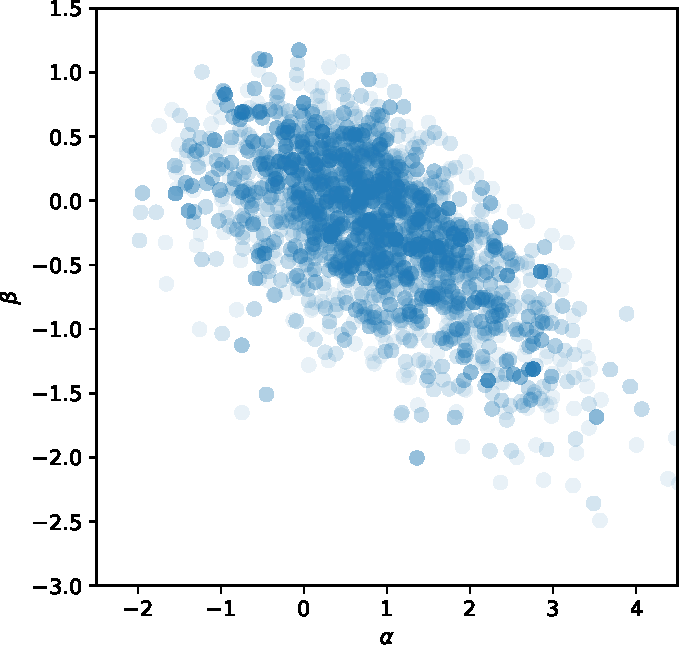
\includegraphics[width=0.5\textwidth]{poisson-posterior}
	\caption{Posterior samples for Poisson regression problem;
          $\thetab_{\mathrm{init}} = (0,0)$.}
	\label{fig:easy}
\end{figure}
      
    \end{solution}

    
\end{exenumerate}


\ex{Mixing and convergence of Metropolis-Hasting MCMC}\label{q:mh_mixing} Under weak conditions, an MCMC
algorithm is an asymptotically exact inference algorithm,
meaning that if it is run forever, it will generate samples that
correspond to the desired probability distribution. In this case, the
chain is said to converge.

In practice, we want to run the algorithm long enough to be able to
approximate the posterior adequately. How long is long enough for the
chain to converge varies drastically depending on the algorithm, the
hyperparameters (e.g.\ the variance \lstinline{vari}), and the target
posterior distribution. It is impossible to determine exactly whether
the chain has run long enough, but there exist various diagnostics
that can help us determine if we can ``trust'' the sample-based
approximation to the posterior.

A very quick and common way of assessing convergence of the Markov
chain is to visually inspect the \emph{trace plots} for each
parameter. A trace plot shows how the drawn samples evolve through
time, i.e.\ they are a time-series of the samples generated by the
Markov chain. Figure~\ref{fig:traceplots} shows examples of trace
plots obtained by running the Metropolis Hastings algorithm for
different values of the hyperparameters \lstinline{vari} and
\lstinline{param_init}. Ideally, the time series covers the whole
domain of the target distribution and it is hard to ``see'' any
structure in it so that predicting values of future samples from the
current one is difficult. If so, the samples are likely independent from
each other and the chain is said to be well ``mixed''.

\begin{exenumerate}
  \item \label{qpt:mh_trace}  Consider the trace plots in Figure~\ref{fig:traceplots}: Is
    the variance \lstinline{vari} used in Figure
    \ref{sfig:traceplot_many_small} larger or smaller than the value of
    \lstinline{vari} used in Figure \ref{sfig:traceplot_many_good}? Is
    \lstinline{vari} used in Figure \ref{sfig:traceplot_many_big}
    larger or smaller than the value used in Figure
    \ref{sfig:traceplot_many_good}?

    In both cases, explain the behaviour of the trace plots in terms of
    the workings of the Metropolis Hastings algorithm and the effect of
    the variance \lstinline{vari}.

    \begin{figure}[p]
      \setcounter{subfigure}{0}% Reset subfigure counter
	\centering
	\subfloat[variance \lstinline{vari}: $1$]{
	  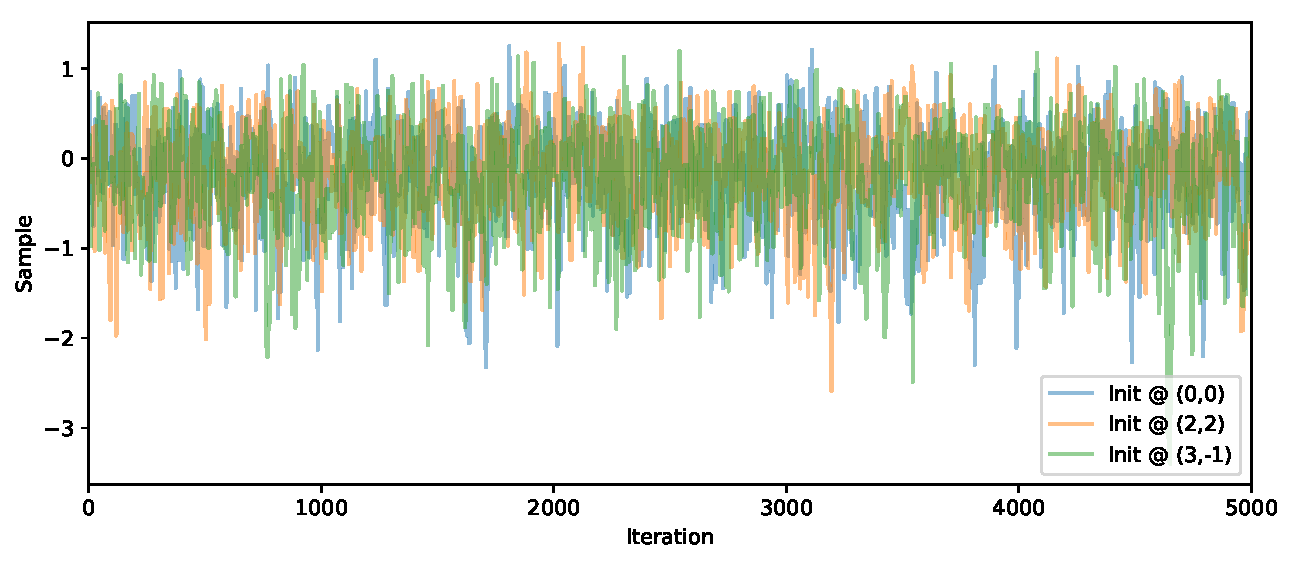
\includegraphics[width=\textwidth]{Q3d_traceplot_stepsize1}
	  \label{sfig:traceplot_many_good}}\\
	\subfloat[Alternative value of \lstinline{vari}]{
	  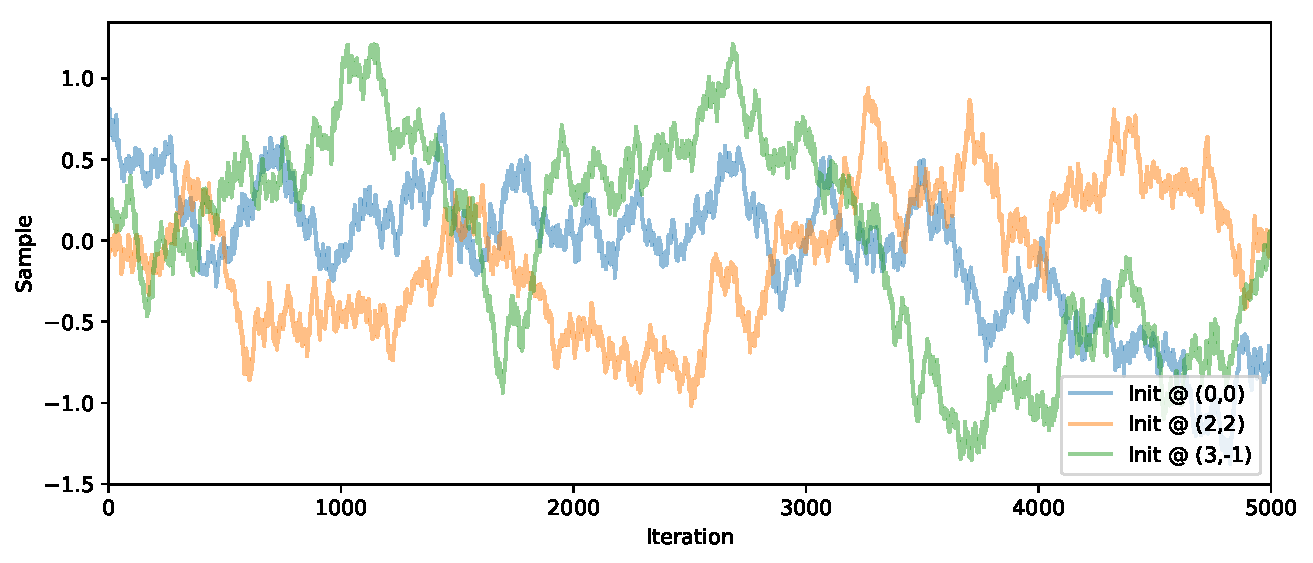
\includegraphics[width=\textwidth]{Q3d_traceplot_stepsize001}
	  \label{sfig:traceplot_many_small}}\\
        \subfloat[Alternative value of \lstinline{vari}]{
	  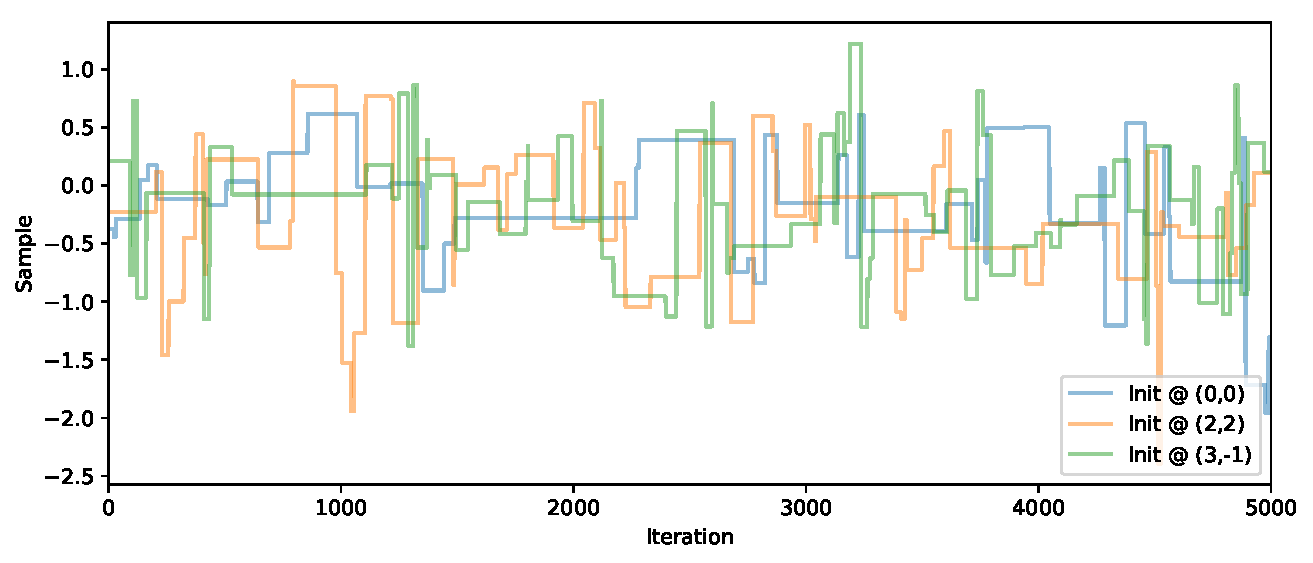
\includegraphics[width=\textwidth]{Q3d_traceplot_stepsize50}
	  \label{sfig:traceplot_many_big}}
	\caption{For Question \ref{q:mh_mixing}\ref{qpt:mh_trace}: Trace plots of the parameter $\beta$ from Question \ref{q:poisson-reg} drawn using Metropolis-Hastings with different variances of the proposal distribution.}
	\label{fig:traceplots}
\end{figure}
%

\begin{solution}

  MCMC methods are sensitive to different hyperparameters, and we
  usually need to carefully diagnose the inference results to ensure
  that our algorithm adequately approximates the target posterior
  distribution.


  \begin{enumerate}[label=(\roman*)]
	
  \item Figure~\ref{sfig:traceplot_many_small} uses a \textit{small}
    variance (\lstinline{vari} was set to $0.001$) . The trace plots show
    that the samples for $\beta$ are very highly correlated and evolve
    very slowly through time. This is because the introduced
    randomness is quite small compared to the scale of the
    posterior, thus the proposed sample at each MCMC iteration will be
    very close to the current sample and hence likely accepted.

    More mathematical explanation: for a symmetric proposal
    distribution, the acceptance ratio $a$ becomes
    \begin{equation}
      a =  \frac{p^*(\thetab^*)}{p^*(\thetab)},
    \end{equation}
    where $\thetab$ is the current sample and $\thetab^*$ is the
    proposed sample. For variances that are small compared to the
    (squared) scale of the posterior, $a$ is close to one and the proposed
    sample $\thetab^*$ gets likely accepted. This then gives rise to the
    slowly changing time series shown in
    Figure~\ref{sfig:traceplot_many_small}.
	
  \item In Figure~\ref{sfig:traceplot_many_big}, the variance is
    larger than the reference (\lstinline{vari} was set to $50$) . The trace
    plots suggest that many iterations of the algorithm result in the
    proposed sample being rejected, and thus we end up copying the
    same sample over and over again. This is because if the random
    perturbations are large compared to the scale of the
    posterior, $p^*(\thetab^*)$ may be very different from
    $p^*(\thetab)$ and $a$ may be very small.

  \end{enumerate}

  \end{solution}

\item In Metropolis-Hastings, and MCMC in general, any sample depends
  on the previously generated sample, and hence the algorithm
  generates samples that are generally statistically dependent. The
  \textit{effective sample size} of a sequence of dependent samples is
  the number of independent samples that are, in some sense,
  equivalent to our number of dependent samples. A definition of the
  effective sample size (ESS) is
  \begin{equation}
    \text{ESS} = \frac{S}{1+ 2\sum_{k=1}^{\infty} \rho(k)}
  \end{equation}
  where $S$ is the number of dependent samples drawn and $\rho(k)$ the
  correlation coefficient between two samples in the Markov chain that
  are $k$ time points apart. We can see that if the samples are
  strongly correlated, $\sum_{k=1}^{\infty} \rho(k)$ is large and the
  effective sample size is small. On the other hand, if $\rho(k)=0$
  for all $k$, the effective sample size is $S$.

$\text{ESS}$, as defined above, is the number of independent
samples which are needed to obtain a sample average that has the same
variance as the sample average computed from correlated samples.

To illustrate how correlation between samples is related to a
reduction of sample size, consider two pairs of samples $(\theta_1,
\theta_2)$ and $(\omega_1, \omega_2)$. All variables have variance
$\sigma^2$ and the same mean $\mu$, but $\omega_1$ and $\omega_1$ are
uncorrelated while the covariance matrix for $\theta_1, \theta_2$ is
$\C$,
\begin{equation}
  \C = \sigma^2 \begin{pmatrix}
    1 & \rho \\
    \rho & 1
  \end{pmatrix},
\end{equation}
with $\rho>0$. The variance of the average $\bar{\omega} = 0.5
(\omega_1+\omega_2)$ is
\begin{equation}
  \var \left( \bar{\omega} \right) = \frac{\sigma^2}{2},
\end{equation}
where the $2$ in the denominator is the sample size.

Derive an equation for the variance of $\bar{\theta} =
0.5(\theta_1+\theta_2)$ and compute the reduction $\alpha$ of the
sample size when working with the correlated $(\theta_1,\theta_2)$. In
other words, derive an equation of $\alpha$ in
\begin{equation}
   \var \left(\bar{\theta}\right) = \frac{\sigma^2}{2/\alpha}.
\end{equation}
What is the effective sample size $2/\alpha$ as $\rho \to 1$?

\begin{solution}
  
  Note that $\E(\bar{\theta}) = \mu$. From the definition of
  variance, we then have
  \begin{align}
    \var(\bar{\theta}) & = \E\left( (\bar{\theta} - \mu)^2\right)\\
    & = \E\left( \left(\frac{1}{2}(\theta_1+\theta_2) - \mu\right)^2\right) \\
    & =  \E\left( \left(\frac{1}{2}(\theta_1-\mu+\theta_2-\mu\right)^2\right) \\
    & =  \frac{1}{4} \E\left( (\theta_1-\mu)^2+(\theta_2-\mu)^2 + 2 (\theta_1-\mu) (\theta_2-\mu)\right) \\
    & =  \frac{1}{4} ( \sigma^2 + \sigma^2 + 2 \sigma^2 \rho) \\
    & =  \frac{1}{4} ( 2\sigma^2 + 2 \sigma^2 \rho) \\
    & =  \frac{\sigma^2}{2} ( 1 + \rho) \\
    & =  \frac{\sigma^2}{2/(1+\rho)}
  \end{align}
  Hence: $\alpha = (1+\rho)$, and for $\rho \to 1$, $2/\alpha \to 1$.
  
  Because of the strong correlation, we effectively only have one sample and not two if $\rho \to 1$.
  
\end{solution}

\end{exenumerate}

